% Root-selected scan021 assembly; pending root approval.
% Exact source and all selected literal components are mapped in scan021_final_source_map.json.
\scanpage{21}
% Reader C, independent scan021. Literal graphical coordinates refer to the original
% 1685 x 2362 scan, top-left origin, x right/y down. Approximate manual paths only;
% no compilation, rendering, metric fitting or image-alignment calculation.
Soit $\alpha_0\in K_1$, je dis que \unsure{l'on a|on a}
\[
% BEGIN C021-G01
\begin{tikzpicture}[x=.085mm,y=-.085mm,baseline={(545,240)},every node/.style={anchor=base west,inner sep=0pt,outer sep=0pt,font=\small},line cap=round,line join=round]
\useasboundingbox (545,140) rectangle (1545,290);
\node at (565,245) {%
% BEGIN C021-G01a
\unsure{\begin{tikzpicture}[x=.085mm,y=-.085mm,baseline={(565,245)},every node/.style={anchor=base west,inner sep=0pt,outer sep=0pt,font=\small},line cap=round,line join=round]
\useasboundingbox (565,150) rectangle (695,260);
% Reading: \widehat{\Sigma}_{\alpha_0}; no written + here.
% Short-head role candidates: Sigma head/retrace | independent upper rule.
\node at (568,245) {$\phantom{\widehat{\Sigma}_{\alpha_0}}$};
\draw (593,174) .. controls (604,170) and (610,165) .. (615,161) -- (626,174);
\draw (574,197) .. controls (588,196) and (604,194) .. (616,194);
\draw (578,202) .. controls (590,205) and (607,207) .. (613,209) -- (575,227) .. controls (590,225) and (608,223) .. (617,224);
\node at (631,240) {$\scriptstyle\alpha_0$};
\end{tikzpicture}}
% END C021-G01a
%
};
\node at (699,239) {$\cap$};
% second roofed Sigma owns its i and + exactly once
\draw (756,172) -- (774,160) -- (789,171);
\draw (743,190) -- (780,187);
\draw (742,197) .. controls (754,201) and (772,201) .. (776,204) -- (742,224) -- (782,224);
\node at (791,239) {$\scriptstyle i$};
\node at (804,201) {$\scriptstyle +$};
\node at (861,229) {$=\varnothing$};
\node at (1090,225) {i.e};
% right first Sigma: its lower return incorporates the alpha body, so no second alpha is printed
\node at (1240,235) {$\phantom{\Sigma_\alpha}$};
\draw (1242,186) -- (1282,183);
\draw (1247,193) .. controls (1262,197) and (1274,199) .. (1280,202) -- (1246,219) -- (1288,216) .. controls (1294,222) and (1291,230) .. (1283,231) .. controls (1273,234) and (1273,223) .. (1288,225);
\node at (1306,245) {$\scriptscriptstyle0$};
\node at (1318,233) {$\cap$};
\draw (1347,185) -- (1378,190);
\draw (1363,190) .. controls (1353,193) and (1343,197) .. (1347,201) .. controls (1352,205) and (1375,207) .. (1371,212) -- (1348,222) .. controls (1361,221) and (1381,220) .. (1383,226);
\node at (1386,226) {$\scriptstyle i$};
\node at (1426,223) {$=\varnothing$};
\end{tikzpicture}
% END C021-G01
\]
(ce qui ach\unsure{è|é|e}vera la d\unsure{è|é|e}monstration, car on aura
\[
% BEGIN C021-G02
\begin{tikzpicture}[x=.085mm,y=-.085mm,baseline={(505,555)},every node/.style={anchor=base west,inner sep=0pt,outer sep=0pt,font=\small},line cap=round,line join=round]
\useasboundingbox (505,385) rectangle (1510,650);
\node at (832,445) {%
% BEGIN C021-M01
\unsure{\begin{tikzpicture}[x=.085mm,y=-.085mm,baseline={(832,445)},every node/.style={anchor=base west,inner sep=0pt,outer sep=0pt,font=\small},line cap=round,line join=round]
\useasboundingbox (832,415) rectangle (890,452);
% Two pale interrupted runs; no character, hand or surface origin assigned.
\draw[gray,line width=.25pt] (838,422)--(844,422) (847,423)--(850,423) (854,423)--(861,424) (864,424)--(871,425);
\draw[gray,line width=.25pt] (842,437)--(847,438) (850,438)--(856,439) (861,440)--(868,441) (873,442)--(880,443);
\end{tikzpicture}}
% END C021-M01
%
};
\node at (520,555) {$U=X\setminus\bigcup_{\alpha\in K}\phantom{\widehat{\Sigma}_\alpha^+}$};
\node[anchor=base west,inner sep=0pt,outer sep=0pt] at (896,535) {$
% A021G05 BEGIN; source bbox=[896, 469, 1018, 563]; source origin=(896,469); baseline y=535; owns: complete Sigma, its separate head, index and any raised sign/hat; no adjoining relation or word
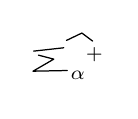
\begin{tikzpicture}[x=.085mm,y=-.085mm,baseline=(A021G05base),line cap=round,line join=round]
\path[use as bounding box] (896,469) rectangle (1018,563);
\coordinate (A021G05base) at (896,535);
\draw[line width=.45pt] (905,504)--(950,499);
\draw[line width=.45pt] (912,510)--(935,516)--(904,534)--(955,533);
\draw[line width=.45pt] (954,488)--(977,477)--(993,489);
\node[anchor=base west,inner sep=0pt,outer sep=0pt] at (960,546) {$\scriptstyle\alpha$};
\node[anchor=base west,inner sep=0pt,outer sep=0pt] at (983,517) {$\scriptstyle+$};
\end{tikzpicture}
% A021G05 END
$};
% The upper and lower brace runs meet at the observed pointed crossing.
\draw (1134,419) .. controls (1134,460) and (1129,523) .. (1124,540) .. controls (1120,548) and (1117,551) .. (1113,552);
\draw (1109,547) .. controls (1114,549) and (1121,558) .. (1119,574) .. controls (1118,596) and (1116,617) .. (1118,630);
\node at (1160,446) {$K=$};
\node at (1260,445) {%
% BEGIN C021-G02a
\unsure{\begin{tikzpicture}[x=.085mm,y=-.085mm,baseline={(1260,445)},every node/.style={anchor=base west,inner sep=0pt,outer sep=0pt,font=\small},line cap=round,line join=round]
\useasboundingbox (1260,398) rectangle (1320,454);
% Complete state candidates: K with head retrace | \deleted{I}K.
\node at (1263,445) {$\phantom{K|\deleted{I}K}$};
\draw (1280,404) -- (1282,444);
\draw (1308,400) .. controls (1302,414) and (1293,425) .. (1282,430) .. controls (1295,432) and (1305,437) .. (1314,446);
\draw (1269,412) -- (1298,411);
\end{tikzpicture}}
% END C021-G02a
%
};
\node at (1316,458) {$\scriptstyle1$};
\node at (1348,447) {$\cup\{i\}$};
% BEGIN B021-G02-cancelled-Sigma
% Complete cancelled lower group; strongest decipherment deleted Sigma_alpha, still qualified.
% Visible geometry owns every old-glyph/cancellation run once; annotation adds no visible strike.
\node[anchor=base west,inner sep=0pt,outer sep=0pt] at (1140,538) {\phantom{$\deleted{\unsure{\Sigma_\alpha}}$}};
\node[anchor=base west,inner sep=0pt,outer sep=0pt] at (1139,540) {\unsure{\begin{tikzpicture}[x=.085mm,y=-.085mm,baseline={(1139,540)},line cap=round,line join=round]
\path[use as bounding box] (1139,484) rectangle (1241,545);
\draw[line width=.35pt] (1152,498).. controls (1165,494) and (1182,493)..(1202,495);
\draw[line width=.35pt] (1158,503)--(1184,512)--(1148,527)--(1207,528);
\draw[line width=.3pt] (1222,529).. controls (1217,536) and (1237,536)..(1233,539).. controls (1224,545) and (1226,536)..(1226,530);
\draw[line width=.45pt] (1139,529)--(1175,491)--(1201,495)--(1146,527);
\draw[line width=.45pt] (1152,527)--(1215,509)--(1169,529);
\draw[line width=.45pt] (1172,530)--(1233,512)--(1209,537)--(1235,537);
\end{tikzpicture}}};
% END B021-G02-cancelled-Sigma
\end{tikzpicture}
% END C021-G02
\]
comme dans le lemme.

Or % BEGIN B021-G03
% Complete selected alternatives: comme | deleted(co) mme | deleted(co) comme | deleted(car) comme.
% Primary keeps the whole group live; the tightly retraced initial cluster leaves the predecessor/live state open.
\unsure{\begin{tikzpicture}[x=.006cm,y=-.006cm,baseline={(560,806)},line cap=round,line join=round]
\path[use as bounding box] (560,773) rectangle (809,813);
\node[anchor=base west,inner sep=0pt,outer sep=0pt] at (560,806) {\phantom{\unsure{comme|\deleted{co}mme|\deleted{co}comme|\deleted{car}comme}}};
\draw[line width=.4pt] (577,779).. controls (566,786) and (561,799)..(569,806).. controls (575,812) and (581,788)..(588,791).. controls (600,801) and (606,790)..(615,795).. controls (624,805) and (603,802)..(593,800)--(574,803);
\draw[line width=.35pt] (637,788).. controls (646,796) and (654,796)..(665,791).. controls (675,795) and (686,789)..(695,787).. controls (708,791) and (709,803)..(697,802).. controls (687,801) and (692,796)..(702,796);
\draw[line width=.35pt] (719,787).. controls (718,796) and (733,792)..(739,787).. controls (747,794) and (756,792)..(765,787).. controls (774,792) and (790,788)..(799,788).. controls (806,789) and (805,794)..(803,795);
\end{tikzpicture}}
% END B021-G03
 on a
\margin{% BEGIN C021-M02
\unsure{\begin{tikzpicture}[x=.085mm,y=-.085mm,baseline={(100,895)},every node/.style={anchor=base west,inner sep=0pt,outer sep=0pt,font=\small},line cap=round,line join=round]
\useasboundingbox (100,878) rectangle (122,899);
\draw[gray,line width=.3pt] (109,891) -- (114,885);
\end{tikzpicture}}
% END C021-M02
}
\[
% BEGIN C021-G03
\begin{tikzpicture}[x=.085mm,y=-.085mm,baseline={(505,930)},every node/.style={anchor=base west,inner sep=0pt,outer sep=0pt,font=\small},line cap=round,line join=round]
\useasboundingbox (505,810) rectangle (1265,1000);
\node at (535,930) {$E_i\subset U_{J,i}=X\setminus$};
% The large union and its high transverse run are each drawn once.
\draw (1015,862) .. controls (1012,894) and (1030,924) .. (1055,923) .. controls (1080,922) and (1085,899) .. (1087,866);
\draw (1008,876) -- (1067,868);
\node at (1015,969) {$\scriptstyle\alpha\in K_0$};
% Complete roofed Sigma group: roof, separate short head, curved body and alpha return, plus.
\node at (1150,924) {$\phantom{\widehat{\Sigma}_\alpha^+}$};
\draw (1166,847) .. controls (1182,845) and (1196,840) .. (1202,836) -- (1218,846);
\draw (1150,875)--(1190,873);
\draw (1159,884) .. controls (1172,887) and (1188,886) .. (1188,891) -- (1155,908) -- (1205,905) .. controls (1212,909) and (1206,917) .. (1191,920) .. controls (1186,916) and (1194,913) .. (1206,913);
\draw (1210,889)--(1227,886) (1220,881)--(1221,895);
\node at (1149,860) {%
% BEGIN C021-M03
\unsure{\begin{tikzpicture}[x=.085mm,y=-.085mm,baseline={(1149,860)},every node/.style={anchor=base west,inner sep=0pt,outer sep=0pt,font=\small},line cap=round,line join=round]
\useasboundingbox (1149,850) rectangle (1162,862);
\fill[gray] (1154,855) circle[radius=.7];
\draw[gray,line width=.2pt] (1155,861)..controls(1153,864)and(1156,866)..(1155,869);
\end{tikzpicture}}
% END C021-M03
%
};
\end{tikzpicture}
% END C021-G03
\]
cela implique que
\[
% BEGIN C021-G04
\begin{tikzpicture}[x=.085mm,y=-.085mm,baseline={(600,1165)},every node/.style={anchor=base west,inner sep=0pt,outer sep=0pt,font=\small},line cap=round,line join=round]
\useasboundingbox (600,1070) rectangle (1290,1210);
\node at (620,1165) {$E_i\subset X\setminus$};
\draw (925,1104)--(951,1085)--(995,1100);
\draw (918,1120)--(957,1117);
\draw (918,1127) .. controls (931,1130) and (951,1131) .. (952,1137) -- (918,1153)--(962,1151);
\node at (979,1168) {$\scriptstyle\alpha_0$};
\draw (978,1114)--(1003,1108) (993,1103)--(995,1124);
\node at (1080,1150) {$=$};
\draw (1142,1110)--(1183,1110);
\draw (1144,1117) .. controls (1162,1121) and (1180,1122) .. (1181,1127) -- (1136,1147)--(1189,1144);
% BEGIN B021-G05-index
\node[anchor=base west,inner sep=0pt,outer sep=0pt] at (1207,1165) {\unsure{\begin{tikzpicture}[x=.085mm,y=-.085mm,baseline={(1207,1165)},line cap=round,line join=round]
\path[use as bounding box] (1207,1132) rectangle (1266,1165);
\node[anchor=base west,inner sep=0pt,outer sep=0pt] at (1207,1165) {\phantom{$\unsure{\alpha_0|\alpha}$}};
\draw[line width=.3pt] (1241,1138).. controls (1236,1158) and (1210,1164)..(1212,1152).. controls (1219,1137) and (1232,1147)..(1237,1153)--(1249,1158).. controls (1263,1159) and (1265,1155)..(1253,1154);
\end{tikzpicture}}};
% END B021-G05-index
\draw (1234,1104) .. controls (1243,1102) and (1254,1100) .. (1261,1105);
\end{tikzpicture}
% END C021-G04
\]
% independent right-margin group; transverse labels run bottom-to-top.
\margin{\unsure{% complete candidates j:e., j.e., i:e., i.e.; two intermediate points present, attachment unresolved
% A021G20 BEGIN; source bbox=[1352, 1129, 1420, 1183]; source origin=(1352,1129); baseline y=1161; owns: complete small marginal lead-in including j dot, two intermediate points, e, final point; diagram outside
\begin{tikzpicture}[x=.055mm,y=-.055mm,baseline=(A021G20base),line cap=round,line join=round]
\path[use as bounding box] (1352,1129) rectangle (1420,1183);
\coordinate (A021G20base) at (1352,1161);
% invisible complete reading/state annotation: \text{j:e.}\mid\text{j.e.}\mid\text{i:e.}\mid\text{i.e.}
\node[overlay,anchor=base west,inner sep=0pt,outer sep=0pt] at (1352,1161) {\phantom{$\text{j:e.}\mid\text{j.e.}\mid\text{i:e.}\mid\text{i.e.}$}};
\draw[line width=.45pt] (1365,1149)..controls(1369,1161)and(1364,1171)..(1357,1176);
\draw[line width=.45pt] (1364,1133)--(1367,1139);
\fill (1378,1155) circle[radius=1.1];
\fill (1381,1161) circle[radius=1.1];
\draw[line width=.45pt] (1395,1144)..controls(1391,1148)and(1392,1155)..(1398,1160);
\fill (1410,1159) circle[radius=1.1];
\end{tikzpicture}
% A021G20 END
}
% A021DG BEGIN; complete marginal diagram; fixed source origin (1435,948).
\diagram{\begin{tikzcd}[ampersand replacement=\&,column sep=0pt,row sep=0pt,execute at end picture={
\begin{scope}[shift={(A021DGanchor.north west)},x=.055mm,y=-.055mm]
\begin{scope}[shift={(-1435,-948)}]
\node[anchor=base west,inner sep=0pt,outer sep=0pt] at (1505,994) {$% A021D01 BEGIN; source bbox=[1505, 957, 1582, 1015]; source origin=(1505,957); baseline y=994; owns: complete Sigma, its separate head, index and any raised sign/hat; no adjoining relation or word
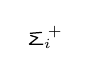
\begin{tikzpicture}[x=.055mm,y=-.055mm,baseline=(A021D01base),line cap=round,line join=round]
\path[use as bounding box] (1505,957) rectangle (1582,1015);
\coordinate (A021D01base) at (1505,994);
\draw[line width=.45pt] (1511,970)--(1537,968);
\draw[line width=.45pt] (1512,975)--(1528,980)--(1509,995)--(1540,995);
\node[anchor=base west,inner sep=0pt,outer sep=0pt] at (1542,1005) {$\scriptscriptstyle i$};
\node[anchor=base west,inner sep=0pt,outer sep=0pt] at (1551,975) {$\scriptscriptstyle+$};
\end{tikzpicture}
% A021D01 END
$};
\node[anchor=base west,inner sep=0pt,outer sep=0pt] at (1603,1000) {$% A021D02 BEGIN; source bbox=[1603, 961, 1665, 1017]; source origin=(1603,961); baseline y=1000; owns: complete Sigma, its separate head, index and any raised sign/hat; no adjoining relation or word
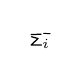
\begin{tikzpicture}[x=.055mm,y=-.055mm,baseline=(A021D02base),line cap=round,line join=round]
\path[use as bounding box] (1603,961) rectangle (1665,1017);
\coordinate (A021D02base) at (1603,1000);
\draw[line width=.45pt] (1611,977)--(1634,976);
\draw[line width=.45pt] (1612,982)--(1627,986)--(1611,1001)--(1635,1001);
\draw[line width=.35pt] (1640,974)--(1655,975);
\node[anchor=base west,inner sep=0pt,outer sep=0pt] at (1636,1010) {$\scriptscriptstyle i$};
\end{tikzpicture}
% A021D02 END
$};
% BEGIN B021-G06-middle-row
\node[anchor=base west,inner sep=0pt,outer sep=0pt] at (1534,1129) {\unsure{\begin{tikzpicture}[x=.055mm,y=-.055mm,baseline={(1534,1129)},line cap=round,line join=round]
\path[use as bounding box] (1534,1090) rectangle (1607,1130);
\node[anchor=base west,inner sep=0pt,outer sep=0pt] at (1534,1129) {\phantom{$\unsure{\Sigma_{i\alpha}\mid\Sigma_{i,\alpha}\mid\Sigma_{\dot\alpha}}$}};
\draw[line width=.4pt] (1538,1095)--(1565,1095);
\draw[line width=.4pt] (1538,1100)--(1560,1106)--(1537,1121)--(1577,1121).. controls (1588,1120) and (1584,1124)..(1585,1127);
\fill (1585,1107) circle[radius=1.3];
\draw[line width=.35pt] (1599,1113).. controls (1591,1125) and (1588,1118)..(1590,1119).. controls (1598,1111) and (1601,1123)..(1605,1126);
\end{tikzpicture}}};
% END B021-G06-middle-row

\node[anchor=base west,inner sep=0pt,outer sep=0pt] at (1518,1251) {$% A021D04 BEGIN; source bbox=[1518, 1206, 1640, 1279]; source origin=(1518,1206); baseline y=1251; owns: complete Sigma, its separate head, index and any raised sign/hat; no adjoining relation or word
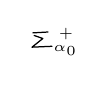
\begin{tikzpicture}[x=.055mm,y=-.055mm,baseline=(A021D04base),line cap=round,line join=round]
\path[use as bounding box] (1518,1206) rectangle (1640,1279);
\coordinate (A021D04base) at (1518,1251);
\draw[line width=.45pt] (1530,1218)--(1565,1216);
\draw[line width=.45pt] (1533,1224)--(1553,1231)--(1528,1251)--(1574,1249);
\node[anchor=base west,inner sep=0pt,outer sep=0pt] at (1578,1260) {$\scriptscriptstyle\alpha_0$};
\node[anchor=base west,inner sep=0pt,outer sep=0pt] at (1590,1228) {$\scriptscriptstyle+$};
\end{tikzpicture}
% A021D04 END
$};
\node[anchor=base west,inner sep=0pt,outer sep=0pt] at (1472,1165) {$% A021D05 BEGIN; source bbox=[1472, 1122, 1498, 1176]; source origin=(1472,1122); baseline y=1165; owns: middle transverse point and curved stroke only; both transverse Sigmas outside
\begin{tikzpicture}[x=.055mm,y=-.055mm,baseline=(A021D05base),line cap=round,line join=round]
\path[use as bounding box] (1472,1122) rectangle (1498,1176);
\coordinate (A021D05base) at (1472,1165);
% invisible complete reading/state annotation: \rotatebox{-90}{$!$}
\node[overlay,anchor=base west,inner sep=0pt,outer sep=0pt] at (1472,1165) {\phantom{$\rotatebox{-90}{$!$}$}};
\fill (1480,1156) circle[radius=.9];
\draw[line width=.4pt] (1487,1145)..controls(1487,1137)and(1487,1131)..(1491,1125);
\end{tikzpicture}
% A021D05 END
$};
\node[anchor=base west,inner sep=0pt,outer sep=0pt] at (1457,1260) {$\unsure{% short detached pale stroke; brace continuation, role, hand and surface origin open
% A021M04 BEGIN; source bbox=[1457, 1244, 1473, 1266]; source origin=(1457,1244); baseline y=1260; owns: short pale stroke below/left of outer brace only
\begin{tikzpicture}[x=.055mm,y=-.055mm,baseline=(A021M04base),line cap=round,line join=round]
\path[use as bounding box] (1457,1244) rectangle (1473,1266);
\coordinate (A021M04base) at (1457,1260);
\draw[gray,line width=.2pt] (1463,1259)--(1466,1247);
\end{tikzpicture}
% A021M04 END
}
$};
\node[anchor=base west,inner sep=0pt,outer sep=0pt] at (1567,998) {$\scriptscriptstyle\text{ou}$};
\node[anchor=base west,inner sep=0pt,outer sep=0pt] at (1528,1063) {$\scriptstyle E_i$};
\node[anchor=base west,inner sep=0pt,outer sep=0pt] at (1515,1181) {$\scriptstyle E_\alpha$};
\begin{scope}[shift={(1435,1285)},cm={0,-1,1,0,(0,0)}]
\draw[line width=.4pt] (58,30)..controls(62,23)and(77,25)..(100,25)..controls(140,26)and(162,45)..(181,40)..controls(200,35)and(205,19)..(196,21)..controls(184,23)and(188,37)..(207,41)..controls(238,46)and(281,45)..(307,35);
\draw[line width=.4pt] (42,77)..controls(61,67)and(83,72)..(112,70)..controls(126,68)and(129,60)..(126,54)..controls(120,48)and(120,59)..(127,65)..controls(144,73)and(170,68)..(192,74)..controls(198,76)and(201,79)..(204,82);
\draw[line width=.4pt] (48,35)--(74,36);
\draw[line width=.4pt] (48,39)--(60,42)--(46,52)..controls(59,52)and(75,56)..(77,56)--(80,64);
\fill (91,45) circle[radius=.8];
\draw[line width=.4pt] (95,33)--(109,34);
\draw[line width=.4pt] (185,46)--(201,51);
\draw[line width=.4pt] (183,50)--(195,55)--(180,63)--(197,66)--(201,74);
\fill (207,62) circle[radius=.8];
\draw[line width=.4pt] (215,56)--(225,61) (221,52)--(219,64);
\end{scope}
\end{scope}
\end{scope}
}]
|[alias=A021DGanchor,anchor=north west,inner sep=0pt,outer sep=0pt]| \phantom{\rule{12.76mm}{18.54mm}}
\end{tikzcd}}
% A021DG END
}
d'autre part $\alpha_0\in K_1$ \unsure{signifie|signifi}
\[
% A021G10 BEGIN; source bbox=[620, 1318, 758, 1414]; source origin=(620,1318); baseline y=1387; owns: complete Sigma, its separate head, index and any raised sign/hat; no adjoining relation or word
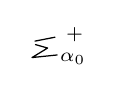
\begin{tikzpicture}[x=.055mm,y=-.055mm,baseline=(A021G10base),line cap=round,line join=round]
\path[use as bounding box] (620,1318) rectangle (758,1414);
\coordinate (A021G10base) at (620,1387);
\draw[line width=.45pt] (637,1349)--(683,1340);
\draw[line width=.45pt] (638,1357)--(666,1365)--(630,1387)--(688,1381);
\node[anchor=base west,inner sep=0pt,outer sep=0pt] at (695,1396) {$\scriptstyle\alpha_0$};
\node[anchor=base west,inner sep=0pt,outer sep=0pt] at (709,1346) {$\scriptstyle+$};
\end{tikzpicture}
% A021G10 END
% A021G11 BEGIN; source bbox=[777, 1327, 845, 1417]; source origin=(777,1327); baseline y=1378; owns: complete crossed inclusion, both strokes; neighbouring Sigmas outside
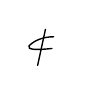
\begin{tikzpicture}[x=.055mm,y=-.055mm,baseline=(A021G11base),line cap=round,line join=round]
\path[use as bounding box] (777,1327) rectangle (845,1417);
\coordinate (A021G11base) at (777,1378);
% invisible complete reading/state annotation: \not\subset
\node[overlay,anchor=base west,inner sep=0pt,outer sep=0pt] at (777,1378) {\phantom{$\not\subset$}};
\draw[line width=.5pt] (837,1348)..controls(813,1348)and(793,1356)..(780,1369)..controls(775,1378)and(797,1379)..(833,1375);
\draw[line width=.5pt] (818,1331)--(800,1414);
\end{tikzpicture}
% A021G11 END
% A021G12 BEGIN; source bbox=[849, 1320, 953, 1401]; source origin=(849,1320); baseline y=1378; owns: complete Sigma, its separate head, index and any raised sign/hat; no adjoining relation or word
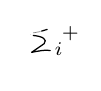
\begin{tikzpicture}[x=.055mm,y=-.055mm,baseline=(A021G12base),line cap=round,line join=round]
\path[use as bounding box] (849,1320) rectangle (953,1401);
\coordinate (A021G12base) at (849,1378);
\draw[line width=.45pt] (881,1328)--(894,1324);
\draw[line width=.45pt] (862,1338)..controls(884,1340)and(895,1347)..(887,1357)--(858,1377)..controls(873,1374)and(893,1370)..(901,1373);
\draw[gray,line width=.25pt] (862,1332)--(878,1329);
\fill[gray] (855,1336) circle[radius=.5];
\node[anchor=base west,inner sep=0pt,outer sep=0pt] at (911,1385) {$\scriptstyle i$};
\node[anchor=base west,inner sep=0pt,outer sep=0pt] at (928,1344) {$\scriptstyle+$};
\end{tikzpicture}
% A021G12 END
\]
ce qui % BEGIN B021-G08
\unsure{\begin{tikzpicture}[x=.006cm,y=-.006cm,baseline={(589,1486)},line cap=round,line join=round]
\path[use as bounding box] (589,1435) rectangle (718,1488);
\node[anchor=base west,inner sep=0pt,outer sep=0pt] at (590,1480) {\phantom{$\deleted{\unsure{\text{impli}|\text{impl.}}}$}};
\fill (597,1447) circle[radius=1.1];
\draw[line width=.35pt] (594,1458).. controls (596,1472) and (610,1465)..(621,1466).. controls (633,1467) and (643,1464)..(652,1467).. controls (661,1468) and (663,1463)..(665,1459);
\draw[line width=.35pt] (669,1438).. controls (670,1456) and (671,1481)..(680,1483).. controls (691,1487) and (678,1462)..(678,1458)--(705,1467);
\draw[line width=.3pt] (699,1450)--(699,1458);
% Two visible cancellation runs; no additional generic strike is drawn.
\draw[line width=.5pt] (592,1468)--(711,1456);
\draw[line width=.35pt] (655,1467)--(704,1471);
\end{tikzpicture}}
% END B021-G08
 signifie aussi que $% BEGIN C021-G08
\begin{tikzpicture}[x=.085mm,y=-.085mm,baseline={(290,1610)},every node/.style={anchor=base west,inner sep=0pt,outer sep=0pt,font=\small},line cap=round,line join=round]
\useasboundingbox (290,1540) rectangle (665,1640);
\node at (300,1610) {$\phantom{\Sigma_i^+\cap\Sigma_\alpha^+=\varnothing}$};
\draw (310,1574)--(350,1568);
\draw (312,1580) .. controls (329,1583) and (344,1587) .. (344,1590) -- (310,1617)--(370,1609) .. controls (376,1610) and (376,1617) .. (379,1620);
\fill (373,1585) circle[radius=.9];
\draw (376,1567)--(399,1568) (385,1556)--(390,1576);
\node at (412,1611) {$\cap$};
\draw (464,1577)--(500,1572);
\draw (465,1580) .. controls (480,1582) and (492,1582) .. (490,1589) -- (467,1604)--(516,1599) .. controls (522,1601) and (512,1609) .. (499,1612) -- (516,1610);
\draw (520,1567)--(537,1566) (526,1560)--(532,1574);
\node at (574,1610) {$=\varnothing$};
\end{tikzpicture}
% END C021-G08
$, cqfd.

\uline{Corollaire du lemme} Pour une classe
\figure{% BEGIN C021-G09
\begin{tikzpicture}[x=.085mm,y=-.085mm,baseline={(180,2340)},every node/.style={anchor=base west,inner sep=0pt,outer sep=0pt,font=\small},line cap=round,line join=round]
\useasboundingbox (180,1810) rectangle (1680,2358);
\node at (319,1852) {%
% BEGIN C021-M05
\unsure{\begin{tikzpicture}[x=.085mm,y=-.085mm,baseline={(319,1852)},every node/.style={anchor=base west,inner sep=0pt,outer sep=0pt,font=\small},line cap=round,line join=round]
\useasboundingbox (319,1838) rectangle (335,1855);
\draw[gray,line width=.25pt] (326,1844)--(326,1848);
\end{tikzpicture}}
% END C021-M05
%
};
\node at (187,2127) {%
% BEGIN C021-M06
\unsure{\begin{tikzpicture}[x=.085mm,y=-.085mm,baseline={(187,2127)},every node/.style={anchor=base west,inner sep=0pt,outer sep=0pt,font=\small},line cap=round,line join=round]
\useasboundingbox (187,2112) rectangle (202,2130);
\fill (194,2121) circle[radius=.7];
\end{tikzpicture}}
% END C021-M06
%
};

% Selected complete A side-rule path; its lower endpoint stops before the physical paper boundary.
% BEGIN A021G25-selected-path
\draw[line width=.4pt] (261,1816)..controls(264,1861)and(266,1954)..(267,2029)..controls(269,2078)and(267,2113)..(260,2157)..controls(257,2178)and(262,2277)..(261,2334);
% END A021G25-selected-path

\node at (300,1915) {$V$ de $\phantom{\Pi_I^{\unsure{\circ|0}}}$, son expression};
\node[anchor=base west,inner sep=0pt,outer sep=0pt] at (490,1907) {$
% A021G22 BEGIN; source bbox=[490, 1863, 597, 1929]; source origin=(490,1863); baseline y=1907; owns: complete Pi, all separated/pale head pieces, lower I and ring; V de and comma outside
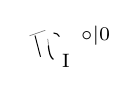
\begin{tikzpicture}[x=.085mm,y=-.085mm,baseline=(A021G22base),line cap=round,line join=round]
\path[use as bounding box] (490,1863) rectangle (597,1929);
\coordinate (A021G22base) at (490,1907);
% invisible complete reading/state annotation: \Pi_I^{\unsure{\circ|0}}
\node[overlay,anchor=base west,inner sep=0pt,outer sep=0pt] at (490,1907) {\phantom{$\Pi_I^{\unsure{\circ|0}}$}};
\draw[gray,line width=.25pt] (493,1875)--(516,1867);
\draw[line width=.35pt] (501,1875)--(509,1906);
\draw[gray,line width=.25pt] (520,1880)--(521,1888);
\draw[line width=.45pt] (521,1890)..controls(522,1901)and(524,1907)..(528,1910);
\draw[line width=.4pt] (529,1871)..controls(533,1871)and(536,1873)..(537,1876);
\node[anchor=base west,inner sep=0pt,outer sep=0pt] at (541,1923) {$\scriptstyle\mathrm I$};
\node[anchor=base west,inner sep=0pt,outer sep=0pt] at (570,1882) {$\scriptstyle\unsure{\circ|0}$};
\end{tikzpicture}
% A021G22 END
$};

\node at (602,2005) {$V=X\setminus$};
\node at (820,1994) {%
% BEGIN C021-G09a
\begin{tikzpicture}[x=.085mm,y=-.085mm,baseline={(820,1994)},every node/.style={anchor=base west,inner sep=0pt,outer sep=0pt,font=\small},line cap=round,line join=round]
\useasboundingbox (820,1935) rectangle (902,2000);
\draw (831,1949) .. controls (831,1972) and (841,1986) .. (861,1986) .. controls (883,1987) and (891,1976) .. (890,1948);
\draw[gray,line width=.3pt] (825,1950) .. controls (825,1964) and (829,1976) .. (837,1981);
\end{tikzpicture}
% END C021-G09a
%
};

\node at (831,2053) {$\scriptstyle\alpha\in K$};
\node[anchor=base west,inner sep=0pt,outer sep=0pt] at (947,1978) {$
% A021G15 BEGIN; source bbox=[947, 1909, 1057, 1995]; source origin=(947,1909); baseline y=1978; owns: complete Sigma, its separate head, index and any raised sign/hat; no adjoining relation or word
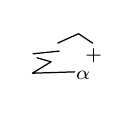
\begin{tikzpicture}[x=.085mm,y=-.085mm,baseline=(A021G15base),line cap=round,line join=round]
\path[use as bounding box] (947,1909) rectangle (1057,1995);
\coordinate (A021G15base) at (947,1978);
\draw[line width=.45pt] (955,1948)--(994,1944);
\draw[line width=.45pt] (961,1954)--(982,1960)--(954,1977)--(1017,1975);
\draw[line width=.45pt] (992,1932)--(1023,1918)--(1044,1932);
\node[anchor=base west,inner sep=0pt,outer sep=0pt] at (1019,1986) {$\scriptstyle\alpha$};
\node[anchor=base west,inner sep=0pt,outer sep=0pt] at (1033,1958) {$\scriptstyle+$};
\end{tikzpicture}
% A021G15 END
$};

\node at (300,2145) {du lemme pr\unsure{ê|é|e}c\unsure{é|è|e}dent est \uline{unique} --};
\node at (315,2231) {on a};
% Main bottom brace: complete visible loop and lower run stopping at the sheet edge.
\draw (489,2227) .. controls (488,2251) and (487,2279) .. (481,2290) .. controls (468,2301) and (460,2286) .. (474,2292) .. controls (487,2297) and (487,2321) .. (493,2346);
\node at (521,2281) {$K=\phantom{\{}\alpha\in I\mid\overline V\cap E_\alpha\ne\varnothing\quad\text{i.e.}\quad$};
% BEGIN B021-G10-set-open
\draw[line width=.35pt] (689,2204).. controls (694,2231) and (697,2248)..(684,2255).. controls (672,2263) and (671,2245)..(686,2253).. controls (696,2264) and (689,2285)..(699,2290)--(706,2284);
% END B021-G10-set-open

\node at (1421,2251) {%
% BEGIN C021-G09b
\begin{tikzpicture}[x=.085mm,y=-.085mm,baseline={(1421,2251)},every node/.style={anchor=base west,inner sep=0pt,outer sep=0pt,font=\small},line cap=round,line join=round]
\useasboundingbox (1421,2180) rectangle (1485,2260);
% The deleted V predecessor is preserved under the live E, not placed twice.
\node at (1425,2251) {$\phantom{\deleted{V}E_\alpha}$};
\draw[gray,line width=.3pt] (1427,2192)--(1437,2247)--(1451,2198);
\draw (1434,2191)--(1440,2248)--(1469,2246);
\draw (1439,2189)--(1460,2186) (1436,2218)--(1464,2215);
\node at (1466,2253) {$\scriptstyle\alpha$};
\end{tikzpicture}
% END C021-G09b
%
};

\node at (1506,2251) {$\cap\dot V\ne\varnothing\phantom{\}}$};
% BEGIN B021-G10-set-close
\draw[line width=.35pt] (1655,2171).. controls (1671,2187) and (1645,2217)..(1654,2233)--(1661,2234).. controls (1666,2264) and (1664,2275)..(1645,2278);
% END B021-G10-set-close

% Final Sigma head/body and signed alpha, all once.
\draw (540,2317)--(579,2314);
\draw (541,2321) .. controls (551,2323) and (570,2326) .. (573,2329) -- (538,2342)--(584,2340);
\node at (595,2344) {$\scriptstyle\alpha$};
\draw (600,2306)--(620,2306) (610,2296)--(611,2317);
\node at (663,2341) {est l'unique comp. de};
\node at (1116,2332) {$X\setminus$};
\draw (1165,2306)--(1188,2309);
\draw (1165,2312) .. controls (1174,2315) and (1187,2317) .. (1187,2321) -- (1167,2331)--(1192,2330);
\node at (1193,2340) {$\scriptscriptstyle\alpha$};
\node at (1240,2334) {contenue dans};
\node at (1554,2325) {$X\setminus V$};
\end{tikzpicture}
% END C021-G09
}
% archive sheet number: 20
